\documentclass{beamer}
\usepackage[utf8]{inputenc}
\usepackage[english]{babel}
\usepackage{amsmath}
\usepackage{amssymb}
\usepackage{fancyhdr}
\usepackage{pgfplots}
\usepackage{setspace}
\usepackage{listings}
\pgfplotsset{compat=1.17} 
\usepackage{enumerate}
\usepackage{algorithm}
\usepackage{algpseudocode}
% \geometry{a4paper} % or letter or a5paper or ... etc
% \geometry{landscape} % rotated page geometry
% \usepackage[margin=2cm]{geometry}
\usepackage{minted}
\usepackage[most]{tcolorbox}
\newtcolorbox{tb}[1][]{%
  sharp corners,
  enhanced,
  colback=white,
  height=6cm,
  attach title to upper,
  #1
}

%These setting will make the code areas look Pretty
\lstset{
	escapechar=~,
	numbers=left, 
	%numberstyle=\tiny, 
	stepnumber=1, 
	firstnumber=1,
	%numbersep=5pt,
	language=C,
	% stringstyle=\itfamily,
	%basicstyle=\footnotesize, 
	showstringspaces=false,
	frame=single,
  upquote=true
}

% created 2022-May-23 %
% Theme choice:
% \usetheme{AnnArbor}
\usetheme{focus}
% Title page details: 
\title{Memory and Pointers in C}
\author{Jonathan Parlett}
\date{\today}

\begin{document}

% Title page frame
\begin{frame}
    \titlepage
	{\bf Memory in C}
\end{frame}

\begin{frame}{What were going to talk about}
	\begin{itemize}[<+->]
		\item Segmentation of memory. How computer memory is allocated by the operating system
		\item What is a segmentation fault
		\item The Stack and the Heap
		\item Malloc, how we request memory from the operating system
		\item Static vs Dynamic Memory, and why you would use one over the other
	\end{itemize}
\end{frame}


\begin{frame}{Segmentation of Memory}
	A big part of C is memory management, so lets discusses how memory is relevant to programs.

	\begin{itemize}[<+->]
		\item Each program has a section of memory allocated to it by the operating system when it is executed. 
		\item Data items and structures such as, arrays, variables and pointers declared in your program are stored in this section of memory.
		\item Programs are not allowed to touch memory outside of what has been allocated by the operating system. If they do a segmentation fault occurs.
		% \item The operating system is also a program, and there is a section of memory that it owns.
	\end{itemize}
\end{frame}

\begin{frame}{Stack and Heap}
	\begin{itemize}[<+->]
	\item The memory allocated to a C program is further divided into the {\bf Stack} and the {\bf Heap}.

	\item 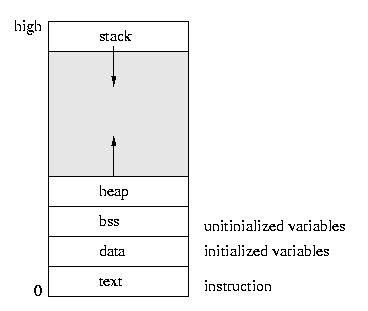
\includegraphics[scale=0.40]{imgs/stackandheap.jpeg}

	\item As data is stored on the Stack it grows down in memory towards the Heap. Increasingly higher valued addresses are used.

	\item As data is stored on the Heap it grows up in memory towards the Stack. Increasingly lower valued addresses are used.

	\end{itemize}
\end{frame}

\begin{frame}{Malloc}
	\begin{itemize}[<+->]
		\item This is a brief overview of malloc, if you don't remember its use from CS265 don't be concerned, we'll cover its use in more detail later.

		\item Malloc is used to request memory from the operating system. Specifically it requests memory from the Heap, not the stack.

		\item \mint{c}|malloc(5)| will return 5 bytes on the heap for example.

		\item We can use the memory given by malloc to store data on the heap.
	\end{itemize}
\end{frame}

\begin{frame}{Static and Dynamic Memory}
	\begin{itemize}[<+->]
		\item All data is stored in memory. This is true for any programming language.
		\item There are a few maintenance tasks that come with using memory.
		\begin{itemize}[<+->]
			\item Requesting it from the operation system I.E {\it malloc}.
			\item Freeing it so it can be reused later.
		\end{itemize}
		\item These tasks are usually handled for you in higher level languages such as python.
		\item The most challenging, and useful thing about C is that you have the ability to fully control memory.
		\item You also have the option of letting the compiler control it for you.
		\item These two dynamics exposed in C are called Static and Dynamic Memory.
	\end{itemize}
\end{frame}

\begin{frame}[fragile]{Static Memory}
	\begin{itemize}[<+->]
		\item Static memory, also called compile time memory is memory that is managed for you, by the compiler.
		\item It uses the Stack for storing data.
		\item When you are declaring variables, arrays, and structs, these data items are stored on the Stack.
		\item The memory is allocated for them by the compiler when they come into scope, and it is deallocated when they fall out of scope.
		\item These variables would be statically allocated on the stack
		\begin{minted}[frame=lines]{c}
int i = 0;
int arr[10];
\end{minted}
	\end{itemize}
\end{frame}



\begin{frame}{Dynamic Memory}
	\begin{itemize}[<+->]
	\item Dynamic memory is the memory you control. You are responsible for requesting it from the operating system, and saying when it is no longer needed so it can be reused.
	\item Dynamic memory uses the Heap.
	\item Dynamic memory is powerful because it allows you to utilize memory programmatically.
	\item You can create data structures that grow and shrink in response to different situations in your program.
	\item It is what allows C to outperform other higher level languages. Greater control means greater optimization opportunities.
	\end{itemize}
\end{frame}

\begin{frame}{Static vs Dynamic Memory}
	\begin{itemize}
		\item Static memory is simpler to use over dynamic memory. No need to worry about allocating or deallocating means less programmer overhead.
		\item Static memory is limited. We cannot adjust the amount of memory allocated for a static structure such as an array. This potentially creates a lot of wasted space.
		\item Dynamic memory is complicated. There is a lot of opportunities to make mistakes.
		\item Dynamic memory is flexible. We can adjust the amount of memory allocated to a structure on the fly. 
		\item Dynamic memory also allows us to be far more efficient then higher level languages.
	\end{itemize}
\end{frame}

\begin{frame}{Thanks For Watching}
	Hopefully you've gained a high level overview of the memory structure of a C program and are prepared to go more in depth into memory and pointers. 
\end{frame}


\end{document}
